\documentclass[11pt,a4paper,oneside]{book}
\usepackage[utf8]{inputenc}
\usepackage{amsmath}
\usepackage{dsfont}
\usepackage{listings}
\usepackage{amsfonts}
\usepackage{amssymb}
\usepackage{tabularx}
\usepackage{enumitem}
\usepackage{algorithm}% http://ctan.org/pkg/algorithm
\usepackage[noend]{algpseudocode}% http://ctan.org/pkg/algorithmicx
\usepackage{parskip}
\usepackage{tikz}
\usepackage[margin=1in]{geometry}
\usepackage{graphicx}
\usepackage{hyperref}
\usepackage{epigraph}
\usetikzlibrary{arrows,positioning} 
\usepackage{subcaption}

\pgfarrowsdeclarecombine{ring}{ring}{}{}{o}{o}

\DeclareMathOperator{\ringarrow}{\raisebox{0.5ex}{\tikz[baseline]{\draw[ring->](0,0)--(2em,0);}}}
\DeclareUnicodeCharacter{00A0}{ }
\tikzset{
    %Define standard arrow tip
    >=stealth',
    %Define style for boxes
    observed/.style={
           circle,
           rounded corners,
           draw=black, thick,
           minimum width=2.2em,
           minimum height=2.2em,
           font=\footnotesize,
           text centered,
           },
     latent/.style={
           circle,
           rounded corners,
           draw=black, thick, dashed,
           minimum width=2.2em,
           minimum height=2.2em,
           font=\footnotesize,
           text centered,
           fill=black!10!white
           },
    target/.style={
           circle,
           rounded corners,
           draw=black, thick,
           minimum width=2.2em,
           minimum height=2.2em,
           font=\footnotesize,
           text centered,
           fill=black!20!white,
           },
    observedrect/.style={
           rectangle,
           rounded corners,
           draw=black, thick,
           minimum width=6em,
           minimum height=2em,
           font=\footnotesize,
           text centered,
           },
     targetrect/.style={
           rectangle,
           rounded corners,
           draw=black, thick,
           minimum width=6em,
           minimum height=2em,
           font=\footnotesize,
           text centered,
           fill=black!20!white,
           },
     empty/.style={
           circle,
           rounded corners,
           minimum width=.5em,
           minimum height=.5em,
           font=\footnotesize,
           text centered,
           },
    % Define arrow style
    pil/.style={
           o->,
           thick,
           shorten <=2pt,
           shorten >=2pt,},
    sh/.style={ shade, shading=axis, left color=red, right color=green,
    shading angle=45 }   
}






\newcommand{\defined}{\vcentcolon =}
\newcommand{\rdefined}{=\vcentcolon}
\newcommand{\E}[1]{\mathbb E\left[{#1}\right]}
\newcommand{\Var}{\operatorname{Var}}
\newcommand{\calF}{\mathcal F}
\newcommand{\sr}[1]{\stackrel{#1}}
\newcommand{\set}[1]{\left\{#1\right\}}
\newcommand{\ind}[1]{\mathds{1}\!\!\set{#1}}
\newcommand{\argmax}{\operatornamewithlimits{arg\,max}}
\newcommand{\argmin}{\operatornamewithlimits{arg\,min}}
\newcommand{\floor}[1]{\left \lfloor {#1} \right\rfloor}
\newcommand{\ceil}[1]{\left \lceil {#1} \right\rceil}
\newcommand{\eqn}[1]{\begin{align}#1\end{align}}
\newcommand{\eq}[1]{\begin{align*}#1\end{align*}}
\newcommand{\Ber}{\operatorname{Bernoulli}}
\newcommand{\bigo}[1]{\mathcal{O}\left( #1 \right)}
\newcommand{\bigotilde}[1]{\tilde{\mathcal{O}}\left( #1 \right)}
\newcommand{\bigtheta}[1]{\Theta\left( #1 \right)}
\newcommand{\bigthetatilde}[1]{\tilde{\Theta}\left( #1 \right)}
\newcommand{\bigomega}[1]{\Omega\left( #1 \right)}

\renewcommand{\P}[1]{\operatorname{P}\left\{#1\right\}}



\author{Finnian Lattimore}
\title{Learning how to act: making good decisions with machine learning}

\begin{document}
\def\ci{\perp\!\!\!\perp} % from Wikipedia
\newtheorem{theorem}{Theorem}[section]
\newtheorem{definition}{Definition}[section]
\maketitle

\epigraph{In vain the grave, with retrospective Eye,
Would from the apparent what conclude the why,
Infer the Motive from the Deed, and show
That what we chanced, was what we meant, to do.}{Alexander Pope}

\chapter{Random Notes}
\begin{itemize}
\item With enough variables it becomes almost a given that we will be able to classify observations by what period they were collected in (eg detecting covariate shift). This means we can conclude the model will fail (when in most cases it will not). Is a form of regularization/reparameterization with an penalty on covariate shift the solution? Focus detection of covariate shift to those variables that actually influence the prediction.

\item If variables are (conditionally) independent they are unlikely to be directly causally linked. 
\end{itemize}


\chapter*{Introduction (3500 words)}


\section*{Motivation}
Many of the most important questions in science and in our personal lives are about the outcomes of doing something. Will asking people to pay upfront at the doctors reduce long term health expenditure? If we developed a drug to suppress particular genes, could we cure MS and would delaying teen-aged pregnancies improve the outcome for their kids.  

These are hard questions because they require more than identifying a pattern in data. Correlation is not causation. Causal inference has proven so difficult using standard methods (such as instrumental variables and propensity scoring) that there is barely any consensus on even enduring questions like the returns to education or the long-term consequences of early life events – like teenage pregnancy, where the variables involved are susceptible to human intuition and understanding. 

We now live in a world of data. Hours of our lives are spent online, where every click can be recorded, tiny computers and sensors are cheap enough to incorporate into everything and the US Institute of Health is considering if all infants should be genetically sequenced at birth. Such data gives us a window into many aspects of our lives at an unprecedented scale and detail but it is messy, complicated and often generated as a by product of some other purpose. It does not come from the controlled world of a randomised experiment. 


Traditional techniques that assume linearity or substantial prior knowledge of causal structure are poorly suited to data sets that may be high dimensional, have non-linear relationships between variables, and where we have limited theory specifying how the variables are related.





Statistical machine learning has been very successful, but generalizing remains very challenging. 


How much data do humans get? 



\paragraph*{Big data and machine learning are a huge deal}

\paragraph*{Data age} Exciting times, larger data sets. Hype, opportunities for Machine learnig. Algorithms beign incorporated everywhere. 

\paragraph*{The end of theory} (it is not) correlation is not enough no matter how many petabytes sit behind it. There are two seperate issues with a correlation only one of which is addressed by larger datasets. One is noise - it may have happened by chance. The other is much more fundamental.

\paragraph*{Large datasets have allowed us to relax assumptions} We can fit more flexible models, rely less on strong parametric assumptions about the form of the curve. 

\paragraph*{Theory is what allows you to extrapolate outside the observed domain (Hal Varian)}

\paragraph*{A cautionary tale} Much hard work remains to be done before we can call and end to theory or the for the automation of science. 

\paragraph*{There is nothing special about humans.} We do have some limited capacity to experiment - but can (or believe we can) draw inferenes about the likely role of variables we have never directy manipulated ourselves. Current ML algorithms are limited. If we ignore this, we will pay a price.

\section*{What is causality and why do we care? (2000 words)}

To explain or to predict \cite{Shmueli2010}
The two cultures \cite{Breiman2001}

\subsection*{Defining causality}
\begin{itemize}
\item widely debated in science and philosophy (FIND SOME REFERENCES)
\item what is explaination?
\item any model that aims to predict the outcome of an action or intervention in a system
\item I do not see the distinction between explaination and (causal) prediction. Explaination is all about the ability to compress and to generalize. The more a model can do this, the more we view as providing an understanding of the why. 
\item mediation?
\end{itemize}

\subsection*{Identifying when we have a causal problem}

\subsubsection*{Examples of typical machine learning probems. Are they causal?}

\begin{itemize}
\item Speech recognition (for systems like Siri or Google)
\item Machine translation 
\item Image classification
\item Forecasting the weather
\item Playing Go 
\item Identiying spam emails
\item Automated essay marking
\item Predicting the risk of death in patients with pnumonia.
\item Predicting who will re-offend on release from prison 
\item Predicting which customers will cease to be your customers
\item Demand prediction for inventory control
\item Predicting who will click on an ad
\item Financial trading
\item Recommending movies
\item Online search
\item Self driving cars
\item Pricing insurance
\end{itemize}

For image recognition, we do not particularly care about building a strong model for exactly how the thing that was photographed translates to the image we see. In fact this is because we already have one. We can be confident that the process will not change. If we develop a discriminative model that is hightly accurate at classifying cats from dogs, we do not care a lot about its internal workings (provided we have strong grounds to believe that the situations in which we will be using our model will match those under which it was trained). Covariate shift clearly comes in here. Because there are areas where mechanisms are understood it is relatively easy to argue that covariate shift is not occuring and that results will be transferable. The mechanism is known but the function may be complex. 

\subsubsection*{What aspects of a problem determine if causal inference is required?}
(When is pure prediction useful?)
\begin{itemize}
\item To decide between actions we only need to rank them (not estimate their actual effect). 
\item The predicted outcome in the absence of an intervention provides a single point. We can use this to find which problems are most serious if left alone - and priortise those for modelling changes. 
\item Any decision we take does not significanly impact the system from which the data was drawn to make it (for repeat decision making)
\item Does acting on the result of the prediction change the predictive distribution p(y|x)? Ie change people's behaviour.
\item Ethics - ... People's viewpoint on if its ok...

\end{itemize}


\section*{Approaches to causality (1000 words)}

\paragraph*{Two broad approaches} 
\begin{itemize}
\item Build a model to map the natural behaviour of the system to what will happen for some action
\item Take the action and see what happens
\end{itemize}

\paragraph*{The first is causal inference}

\paragraph*{The second is reinforcement learning}

\paragraph*{Both generalize from randomized experiment} Reinforcment learning to sequential decisions, causal inference to non-experimental conditions

\paragraph*{Both approaches involve assumptions} the latter that we can group context and actions.

\paragraph*{Limitations of causal inference}

\paragraph*{Limitations of experimets} What are the issues with standard randomized experiments?

\chapter*{Causal models (3000 words)}

Causal inference aims to infer the outcome of an intervention in a system from data obtained by observing (but not intervening in) the system. To do this we need terminology to describe actions and how we anticipate the system should respond to them. Three key approaches have emerged; counterfactuals, structural equation models and causal bayesian networks. In this chapter we describe these approaches, examine what problems they allow us to solve and the assumptions they rely on and discuss their differences.

\subsection*{Counterfactuals}
Counterfactuals (or potential outcomes) are a way of describing distributions under different actions that were developed from the starting point of generalizing randomized experiments. 


There are philosophical objections (references) to counterfactuals because of the way the describe alternate universes that were never realized and are not empirically testable (example). 

For interventional queries, of the form; what is the is the probaiblity distribution for the variable Y if we intervene to set X = x, and the system is otherwise unchanged? Counterfactuals are a short hand. They say what is the distribution of Y had X = x (regardless of the value X actually took).


\subsection*{Causal graphical models}
Although seemingly simplistic, the notion of hard interventions is surprisingly powerful. 

A complaint leveled against this view point of causality is that the 'surgery' is too precise and that, in the real world, any intervention will effect many variables (eg Cartwright 2007). However, 

Provides an explicit mechinism to map knowelede from one setting to another. 

A fully observed causal bayesian network allows asymtoptic point estimates of the causal effect of any intervention (assuming positive density). 


\subsection*{Structural Equation models}


\subsection*{Comparing and unifying the models}
Representation equivelent for interventional queries
This means it is straightforward to take the best elements of work done in any of the frameworks. For example, draw a graphical network to determine if a problem is identifiable and which variables we need to adjust for to obtain an unbiased causal estimate. Then use propensity scores or ... to estimate that effect. Alternatively, make parametric assumptions, to make the problem into a structural equation model. 

SWIGs \cite{Richardson2013}
\cite{Dawid2000} Causal inference without counterfactuals

Determinisim inherent in counterfactuals and SEMs.

Key issue is that we can't observe the joint distribution over $Y_t$ and $Y_c$ even with randomized experiment. 

Suppose the counterfactuals $Y_t$ and $Y_c$ are jointly normal (with equal variance),
\eq{
P(Y_t,Y_c) \sim N()
}

then their difference is also normal,

\eq{
P(\tau) = N(\mu_t - \mu_c,2\sigma^{2}(1-\rho))
}

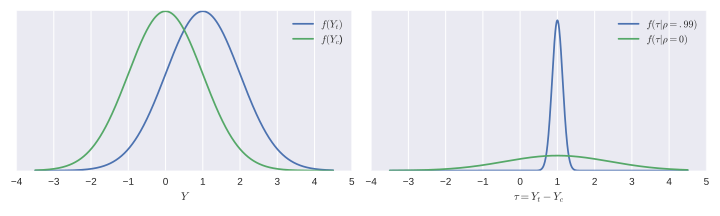
\includegraphics[scale=.6]{figures/counterfactual_nonidentify.pdf}

The variance of $\tau$ is not identifiable, even from experimental data. But it seems on the face of it relevent to our decision making. If the example above, if $\rho = 1$ then almost everyone benifits slightly from the treatment. However if $\rho=0$, there is a wide range, with some people benifiting a lot and others suffering significant harm.  

Note that we can bound this counterfactual distribution based on the variance of the observed interventional distributions. 

Can these issues be resolved by considering personalized causal effects as random variables and avoiding counterfactuals?

Counterfactuals make a natural way to talk about causal effects in natural language. They could be seen as a short hand for projecting the world forward, holding everything else constant. An (impresise) way of expressing that we wish to consider the effect of only a single change. 

What assumptions are required for the kind of counterfactual analysis like X would have been higher had B ...?

\subsection*{What does a causal model give us? Resolving Simpson's paradox}

Simpsons paradox



\subsubsection{A translator from graphical independence to counter factual statements}
\subsection*{Defining causal effects} Summarising the difference between two distributions. There is no one answer. \cite{Janzing2013}

\chapter*{Two key questions (5000 words)}

We can rougly categorize the problems studied within causal inference into two groups, causal effect estimation and causal discovery. In causal effect estimation we assume (at least implicitly) that key aspects of the causal graph are known. The goal is then to estimate the causal effect of some action or range of actions. WHERE DOES MEDIATION FIT IN? THIS IS ALREADY HUGE, and is central to 1000 of papers published each year. Causal discovery aims to leverage much broader assumptions to learn the stucture of causal graph from data. THIS IS THE AUTOMATION OF SCIENCE.

 
\section*{Causal Inference} 
\paragraph*{You are willing to assume the causal graph}
\paragraph*{extremely widely appliled} Implicitly accounts 10,000 of studies in phycology, medicine, business, etc. 

\subsection*{Identifiability}
\paragraph*{Definition:asymptopic point estimate is possible, without parametric assumptions}
\paragraph*{Under what conditions in is the problem solveable}
\subsubsection*{The Do Calculus}


\subsection*{Estimation}
\cite{Imbens2004} Review of non-parametric estimation
\paragraph*{How well do we actually do with finite datasets?}

\paragraph*{When is regression causal?}


\subsection*{Non identifiable queries}

\subsubsection*{Parametric assumptions}
eg linearity

\subsubsection*{Bounds}
\paragraph{Instrumental variables are an example}


\section*{Causal Discovery}
It is possible to infer some aspects of causal structure with very general assumptions. The set of conditional independences in a non-experimental data set indicates some causal structures are more likely than others. In addition, there are subtle asymmetries in the relationship between the joint distribution of cause and effect and the distributions of cause given effect and effect given cause. These clues are the key to causal discovery algorithms, which attempt to learn causal structure from non-experimental data. 

\paragraph*{You want to learn the graph}
\paragraph*{Equates to the aim of automating scientific discovery}
\paragraph*{Increadibly hard}
\paragraph*{Methods can also be divided into contraint based and search and score}
\subsection*{Discovery with Conditional independence}
If variables are (conditionally) independent they are unlikely to be directly causally linked. 
\subsection*{Discovery with Functional Models}
\subsection*{Granger causality}

\chapter*{The interventionalist viewpoint (5000 words)}

Instead of trying to infer the outcome of an intervention in a system from passive observations we could just try the intervention and see what happens.

Randomization is not a requirement. -> control over treatment assignment is.

Experiments, bandits, reinforcement learning

\paragraph*{internal validity} Are differences in treatment and control groups down to intervention or the result of bias? 

\paragraph*{external validity} Are the results of the study applicable to the broader population of interest.

\paragraph*{Fundamental role of randomization}


\paragraph*{Feature selection} Is it even more important here? How do algorithms degrade as irrelevent features are added? In the supervised vs the RL setting? What would be a fair comparison?

Image of randomization breaking any confounding links

Randomization does not ensure target and control group are exactly alike. The more features or variables you include, the more likely that there will be a significant difference across at least one variable. But the within group variance also increases, the net effect is that it becomes harder to draw a conclusion but not more biased. 

\paragraph*{Practical limitations of experimentation} Failure to generalize. Transportability, imperfect compliance. Too many contexts.

What is the role of randomization? How do bandits algorithms work despite being only partially randomized? 
What else can you do to improve randomized studies (variance reduction, lower regret).

\section*{Multi armed bandits}
\paragraph*{Motivation} Why we need to extend from simple randomized experiment.

\subsection*{Regret}
\paragraph*{Relationship to Markov decision processes}
\subsection*{The exploration/exploitation trade-off}

\subsection*{Contexual bandits}


\subsection*{Dynamic Systems}
\begin{itemize}
\item An explicit model of actions in a partially known system (eg HMM)
\item Feynman-Kac Lemma; Solving a PDE can be converted to a stochastic process
\end{itemize}


\chapter*{Causal Bandits: Unifying the approaches (5000 words)}

\subsection*{Learning from log data}



\chapter*{Causal Inference \& Machine Learning (5000 words)}
A more detailed discussion on where causal inference sits within machine learning and what it can offer.



\section*{Different approaches}
\paragraph{The two cultures}


\subsubsection*{Translating terminology}
Economist -> ML

\section*{Challenges for the Machine learning approach}
\subsection*{No cross validation}
\paragraph*{The challenge of model selection}
\paragraph*{Does predictive accuracy indicate a good causal model?}
\subsection*{Less large, real world datasets}
\paragraph*{The dearth of experimental data}
\subsubsection*{Data for testing causal models}
Simulators. Open competitions. Converting other data sets. Existing data sets.

\paragraph*{Are models that predict better more likely to be the correct model?}
For polynomials, if you know the data was generated by a higher order polynomial, you may still be better of predicting it with a lower order one.

\section*{Relation to other areas of ML}
\subsection*{Covariate shift}
\subsection*{Generalizability}
\paragraph*{Invariants}
\paragraph{more stable} Variables causally directly causally related to the outcome (either causes or effects) should be more stable predictors over time. The assumption is there are less places for change to come in. 

\paragraph{change input distribution}If a feature is a cause of an outcome then changing the input distribution over that feature won't break the model. If its an effect it could.

\paragraph{feature selection} The direct causes (and effects) of a variable of interest make up a sufficient set for prediction (is this true)? This may be a reason for using structure learning type algorithms even if you are simply doing prediction.
\subsection*{Interpretabilty}
\paragraph*{Interpretable models as proxies for causal models} Let the human do the work. If we know the training and test data will be sampled from different distributions, knowing what the features that the model is looking at are, allows people use their background understanding of the world to evaluate whether or not those features are likely to be transferable to the test domain. 

\paragraph*{Causal models are more interpretable?}

A desire for interpretability indicates that something has been left out of the loss function. 

One form of interpretability gives people insight into what the features are that the model is relying on.

Specifically, people can
\begin{itemize}
\item rule out many possible features as highly unlikely to be relevent to a problem
\end{itemize}

People have access to a lot of detailed prior knowledge.  

http://www.news.com.au/finance/money/costs/insurance-companies-secrets-spilt/news-story/f6ef17ae73e3a5636343845666532b91 insurance decisions voodoo because of lack of transparancy and absense of obvious causal link. Claim: People are more comfortable with desicion making on the basis of factors they believe to be causally relevet.

\subsection*{Transfer Learning}
find a feature representation in which $P(Y|X)$ is the same in many different domains (or stable over time). Causal models predict the outcome of actions. We could directly take these actions and learn $P(Y|a,X)$ for every $(a,X)$ but, in reality, no two situations (or actions) are exactly alike. So we have to make representations such that things are stable. 

This is tightly related to generalizability. If we take a person undergoing a medical test, we might describe the situation by the year and location, the person's age, gender, heart rate, medical condition and test results. We don't include , the color of the doctors shirt, the size of the room, ...

For example, in the advertising setting, we want to know how our on expenditure on paid search ads is linked to sales. However, this relationship may be very unstable over time because the ad slots are sold at auction. The amount we have to pay to obtain a given position for keyword depends crucially on the amount our competitors are bidding for that keyword. However, the relationship between displaying the ad at a particular position and the probability that someone clicks it an then makes a purchase may be much more consistent. 

\subsection*{Fair Machine Learning}
\paragraph*{Exchangeability of people} Is there any connection to the concept of imagining you could be born in any position and designing ethics from there?
\begin{itemize}
\item what determines what attributes we deam worthy of protection (eg race, gender, sexuality)
\item what do we protect (and what exceptions do we give)?
\item Do we think it is bad to select on the basis of protected attributes not directly related to desired outcome?
\item Do we think it is bad to select in a way that has a disparate impact on a minority/disadvantaged group.
\end{itemize}


\subsection*{Causal inference with Bayesian Graphical models}

\subsubsection*{The likelyhood principle}
Look at some examples from the stan book.

Both frequentist and bayesian methods can be used to approach problems of infering the outcome of an intervention. However, Bayesian modelling allows you to very naturally encode aditional assumptions and causal prior knowledge. This seems especially critical for problems that are not non-parametrically identifiable. 

In the same way that regression may be either causal or non causal, depending on what interpretation and assumptions the researcher places on the equations relating the variables, Bayesian models may or may not be interpretable causally.  

Is setting certain priors equivelent to conditioning? How must the model be set up to ensure unbiased causal estimates (in what way are the assumptions different to if you are using bayesian estimation techniques for prediction?)

\chapter*{Conclusions (1000 words)}

\section*{Open questions}
\paragraph{Cycles} - a huge issue. Not covered by Pearl,Rubin etc. 

Places to look, statistical control theory, etc. any interesting papers along these lines?


\bibliographystyle{apalike}% Select the citation style e.g. ieeetr
\bibliography{../library}% write the directory to the .bib file
\end{document}




